\documentclass[11pt]{report}

% Paquetes y configuraciones adicionales
\usepackage{amsmath, amsthm, amssymb} % Paquetes matemáticos
\usepackage[utf8]{inputenc} % Codificación .tex
\usepackage[T1]{fontenc} % Codificación .pdf
\usepackage{graphicx}
\usepackage[export]{adjustbox}
\usepackage{caption}
\usepackage{float}
\usepackage{titlesec}
\usepackage{geometry}
\usepackage[hidelinks]{hyperref}
\usepackage{titling}
\usepackage{titlesec}
\usepackage{parskip}
\usepackage{wasysym}
\usepackage{tikzsymbols}
\usepackage{fancyvrb}
\usepackage{xurl}
\usepackage{hyperref}
\usepackage{subcaption}
\usepackage{listings}
\usepackage{xcolor}
\usepackage[spanish]{babel}


\newcommand{\subtitle}[1]{
  \posttitle{
    \par\end{center}
    \begin{center}\large#1\end{center}
    \vskip0.5em}
}

% Configura los márgenes
\geometry{
  left=2cm,   % Ajusta este valor al margen izquierdo deseado
  right=2cm,  % Ajusta este valor al margen derecho deseado
  top=3cm,
  bottom=3cm,
}

% Configuración de los títulos de las secciones
\titlespacing{\section}{0pt}{\parskip}{\parskip}
\titlespacing{\subsection}{0pt}{\parskip}{\parskip}
\titlespacing{\subsubsection}{0pt}{\parskip}{\parskip}

% Redefinir el formato de los capítulos y añadir un punto después del número
\makeatletter
\renewcommand{\@makechapterhead}[1]{%
  \vspace*{0\p@} % Ajusta este valor para el espaciado deseado antes del título del capítulo
  {\parindent \z@ \raggedright \normalfont
    \ifnum \c@secnumdepth >\m@ne
        \huge\bfseries \thechapter.\ % Añade un punto después del número
    \fi
    \interlinepenalty\@M
    #1\par\nobreak
    \vspace{10pt} % Ajusta este valor para el espacio deseado después del título del capítulo
  }}
\makeatother

% Configura para que cada \chapter no comience en una pagina nueva
\makeatletter
\renewcommand\chapter{\@startsection{chapter}{0}{\z@}%
    {-3.5ex \@plus -1ex \@minus -.2ex}%
    {2.3ex \@plus.2ex}%
    {\normalfont\Large\bfseries}}
\makeatother

\definecolor{mygreen}{RGB}{0,128,0}  % Definir el color verde (0,128,0)
\definecolor{myblue}{RGB}{0,0,128}   % Definir el color azul (0,0,128)

\begin{document}

% Portada del informe
\title{Informe de prácticas}
\subtitle{Robótica Computacional}
\author{Cheuk Kelly Ng Pante (alu0101364544@ull.edu.es)}
\date{\today}

\maketitle

\pagestyle{empty} % Desactiva la numeración de página para el índice

% Índice
\tableofcontents

% Nueva página
\newpage

\pagestyle{plain} % Vuelve a activar la numeración de página
\setcounter{page}{1} % Reinicia el contador de página a 1

% Secciones del informe
% Capitulo 1
\chapter{Cinematica Directa}
La cinemática directa es una rama de la robótica y la mecánica que se ocupa de la relación entre los movimientos
de los eslabones de un robot y las variables que los controlan. En otras palabras, la cinemática directa es el
problema de encontrar la posición y orientación del extremo del robot, dado el conjunto de parámetros que
definen las posiciones y orientaciones de todos los eslabones.

Para explicar la cinemática directa, se utilizará el sistema de coordenadas de Denavit-Hartenberg (DH). El sistema
de coordenadas de Denavit-Hartenberg es un sistema de coordenadas utilizado para modelar cinemática directa e
inversa de robots articulados. El sistema de coordenadas de Denavit-Hartenberg se basa en cuatro parámetros
asociados a cada articulación. Estos parámetros son:
\begin{itemize}
  \item $d_i$: Distancia entre los ejes $z_{i-1}$ y $z_i$ a lo largo del eje $x_i$.
  \item $\theta_i$: Ángulo entre los ejes $z_{i-1}$ y $z_i$ alrededor del eje $x_i$.
  \item $a_i$: Distancia entre los ejes $x_{i-1}$ y $x_i$ a lo largo del eje $z_{i-1}$.
  \item $\alpha_i$: Ángulo entre los ejes $x_{i-1}$ y $x_i$ alrededor del eje $z_{i-1}$.
\end{itemize}

Los parámetros DH se pueden calcular segun la tabla siguiente:
\begin{table}[H]
  \centering
  \begin{tabular}{|c|c|c|c|}
    \hline
    \textbf{}           & \textbf{A}                 & \textbf{B}                 & \textbf{C}         \\ \hline
    \textbf{$d_i$}      & \texttt{$O_{i-1}$}         & \texttt{$Z_{i-1}\cap X_i$} & \texttt{$Z_{i-1}$} \\ \hline
    \textbf{$\theta_i$} & \texttt{$X_{i-1}$}         & \texttt{$X_{i}$}           & \texttt{$Z_{i-1}$} \\ \hline
    \textbf{$a_i$}      & \texttt{$Z_{i-1}\cap X_i$} & \texttt{$O_{i}$}           & \texttt{$X_{i}$}   \\ \hline
    \textbf{$\alpha_i$} & \texttt{$Z_{i-1}$}         & \texttt{$Z_{i}$}           & \texttt{$X_{i}$}   \\ \hline
  \end{tabular}
  \caption{Parámetros DH}
\end{table}

Para la explicación de la cinemática directa, se utilizará el manipulador 3:
\begin{figure}[H]
  \centering
  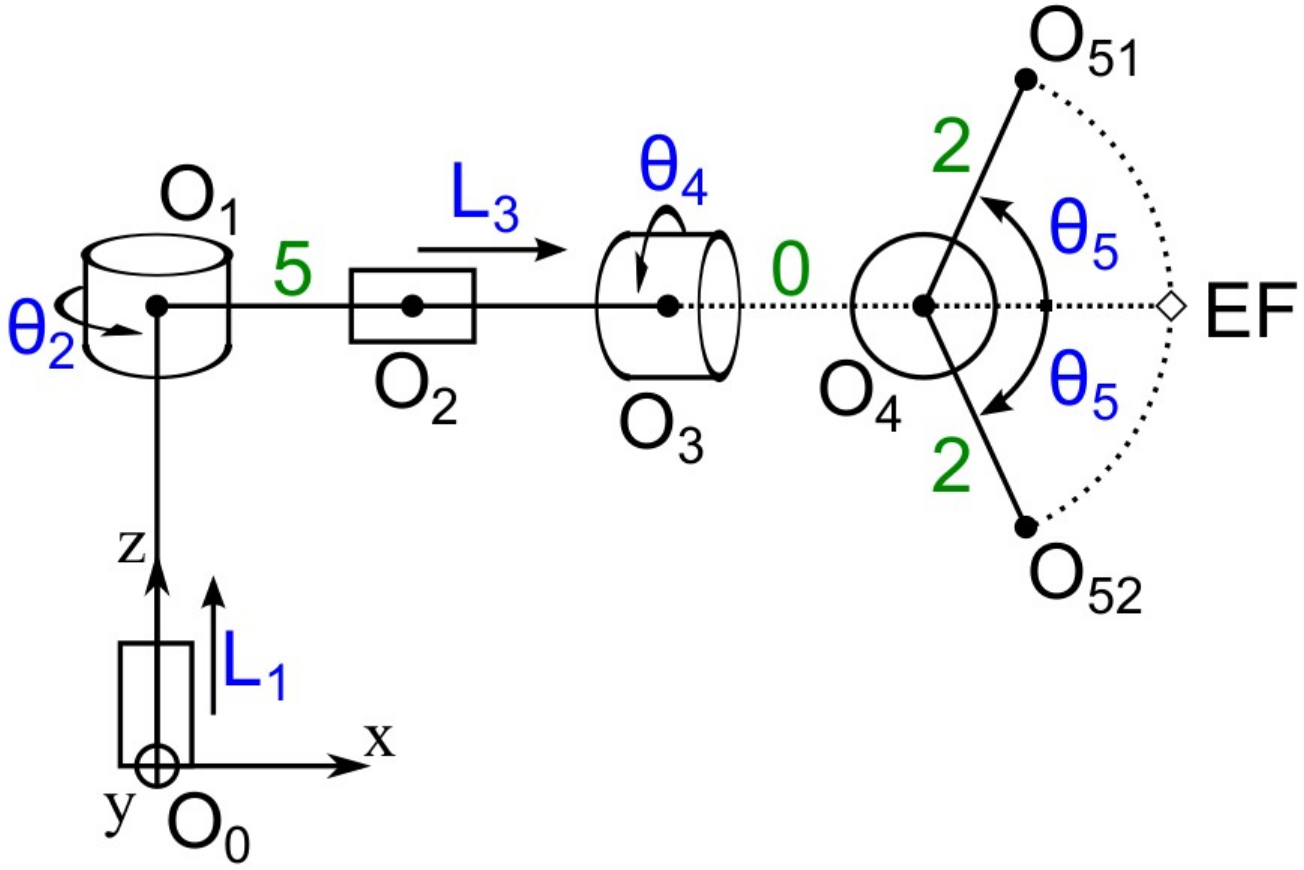
\includegraphics[scale=0.24]{img/manipulador.png}
  \caption{Manipulador ejemplo}
\end{figure}
Para calcular la cinemática directa, primero vamos a calcular los parámetros DH:
\begin{figure}[H]
  \centering
  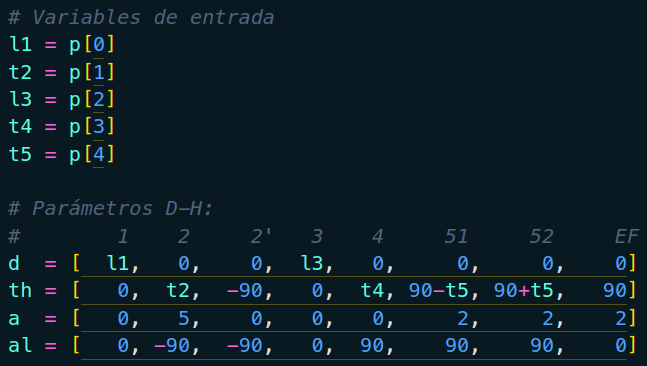
\includegraphics[scale=0.4]{img/parametros_dh.png}
  \caption{Parámetros DH del manipulador 3}
\end{figure}

Como se puede observar en la figura 1.2, antes de calcular los parámetros DH, se ha
asignado unas variables de entrada, estas corresponden a los ángulos de las articulaciones del manipulador
y estas son los valores que se introducen al ejecutar el programa. Por ejemplo, si lo ejecutamos de la siguiente
manera:
\begin{verbatim}
$ python3 ./cinematica_directa 5 0 5 90 45
\end{verbatim}

el resultado de la cinemática directa sería la siguiente:
\begin{figure}[H]
  \centering
  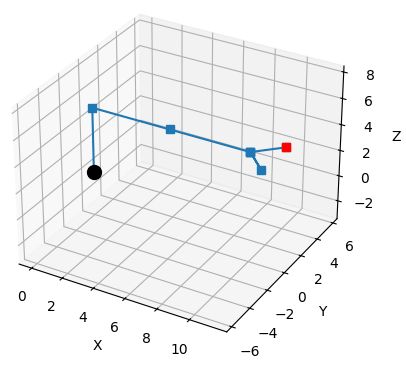
\includegraphics[scale=0.7]{img/cinematica_directa.png}
  \caption{Cinemática directa del manipulador 3}
\end{figure}

\newpage

Después, se calculado la matriz de transformación de cada articulación para este manipulador:
\begin{figure}[H]
  \centering
  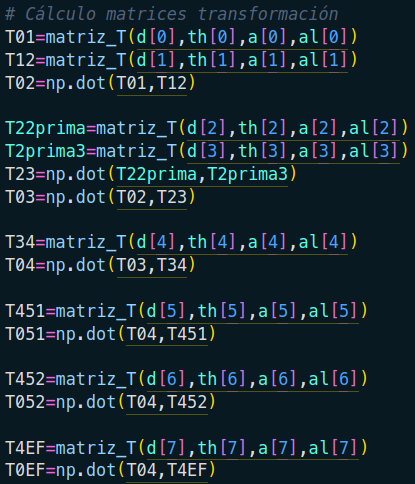
\includegraphics[scale=0.5]{img/matriz_transformacion.png}
  \caption{Matriz de transformación del manipulador 3}
\end{figure}

Luego, la transformación de cada articulación, especificando los datos de la tabla de Denavit Hartenberg especificadas en la figura 1.2:
\begin{figure}[H]
  \centering
  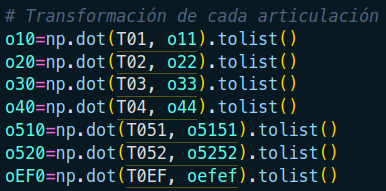
\includegraphics[scale=0.5]{img/transformacion_articulacion.png}
  \caption{Transformación de cada articulación del manipulador 3}
\end{figure}

Y por último, el resultado de la cinemática directa del manipulador 3:
\begin{figure}[H]
  \centering
  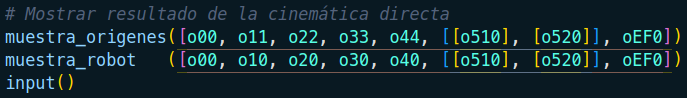
\includegraphics[scale=0.5]{img/resultado_cd.png}
  \caption{Cinemática directa del manipulador 3}
\end{figure}

\newpage

\chapter{Cinematica Inversa}
La cinemática inversa es una rama de la robótica y la mecánica que se ocupa de la relación entre los movimientos
de los eslabones de un robot y las variables que los controlan. En otras palabras, la cinemática inversa es el
problema de encontrar el conjunto de parámetros que definen las posiciones y orientaciones de todos los eslabones,
dado la posición y orientación del extremo del robot.

La cinemática inversa puede ser un problema complejo debido a la presencia de restricciones y limitaciones física
del robot, como por ejemplo, limites de movimientos de las articulaciones, colisiones o singularidades.

En la práctica de la cinemática inversa, se ha de calcular la distancia que debe extenderse una articulación prismática
situada en el punto $O_i$, de tal forma que el punto final del robot $O_n$ se acerque tanto como sea posible a la posición
objetivo R.

El acercamiento solo puede hacerse en la dirección de extensión $L_i$, que se puede calcular como un angulo de $w$ que define
la rotación respecto al eje x absoluto. El angulo $w$ se puede calcular como:
\begin{equation*}
  \color{blue}\omega\color{black} = \sum_{j = 0}^{\color{blue}i\color{black}} \theta_j
\end{equation*}

Usando el producto escalar se puede proyectar el vector que $O_n$ hasta $R$ sobre la dirección de extensión de la articulacion
obteniendo así la distancia $d$:
\begin{equation*}
  \color{green} \mathbf{d} \color{black} =
  \begin{bmatrix}
    \cos(\color{blue}\omega\color{black}) \\
    \sin(\color{blue}\omega\color{black})
  \end{bmatrix}
  \cdot (\color{red}R\color{black}- \color{red}\text{ON}\color{black})
\end{equation*}

Por tanto, el valor de $L_i$ tras cada iteración pasa a ser:
\begin{equation*}
  \color{green} \mathbf{L_i} \color{black} +
  \begin{bmatrix}
    \cos(\color{blue}\omega\color{black}) \\
    \sin(\color{blue}\omega\color{black})
  \end{bmatrix}
  \cdot (\color{red}R\color{black}- \color{red}\text{ON}\color{black}),\ \ \ con \ 
  \color{blue}\omega\color{black} = \sum_{j = 0}^{\color{blue}i\color{black}} \theta_j
\end{equation*}

Para calcular la cinemática inversa en el script en \emph{Python} lo haremos con el algoritmo Cyclic Coordinate Descent (CCD).
Y antes de empezar a desarrollar el algoritmo CCD, se ha de definir primero los valores articulares para la cinematica directa.
Para ello se han definido unas listas con los valores articulares de cada articulación del robot y estos valores articulares
se han definido para que el robot no sobrepase los límites de las articulaciones, limite superior e inferior. Y luego, con 
otra lista se van a diferenciar entre una articulación rotacional y una prismática.

\begin{figure}[H]
  \centering
  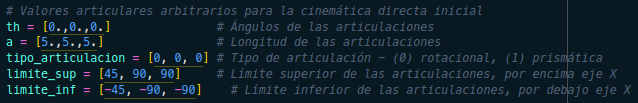
\includegraphics[scale=0.7]{img/listas_ci.png}
  \caption{Listas de límites de las articulaciones del robot}
\end{figure}

\newpage

Después, ya diferenciando los valores articulares, en el bucle principal calculamos $\omega$ que para la articulación rotacional 
calculamos los vectores $V_1$ y $V_2$, que representan las diferencias de posición entre los puntos de interés. Para el vector $V_1$ 
es la diferencia entre el punto final del robot y el objetivo y para el vector $V_2$ es la diferencia entre el punto final del robot 
y el punto de interés. Una vez calculados los vectores, calculamos los angulos entre los vectores $V_1$ y $V_2$ y estos angulos se 
suman a la variable $\theta$ de la articulación rotacional haciendo la diferencia entre los angulos de los vectores $V_1$ y $V_2$.
Y en el caso de la articulación prismática será la suma de todas las $\theta$ hasta la actual (inclusive) y después se calcula la
la proyección escalar del vector que va desde el punto final del robot hasta el objetivo sobre la dirección de extensión de la articulación
prismática. 

Después, hay que prevenir que el robot no sobrepase los límites de las articulaciones, por lo que se ha de comprobar es la posicion actual si es superior o inferior a los límites y si 
es así la posición pasará a ser la del propio limite, sea superior o inferior.
\begin{figure}[H]
  \centering
  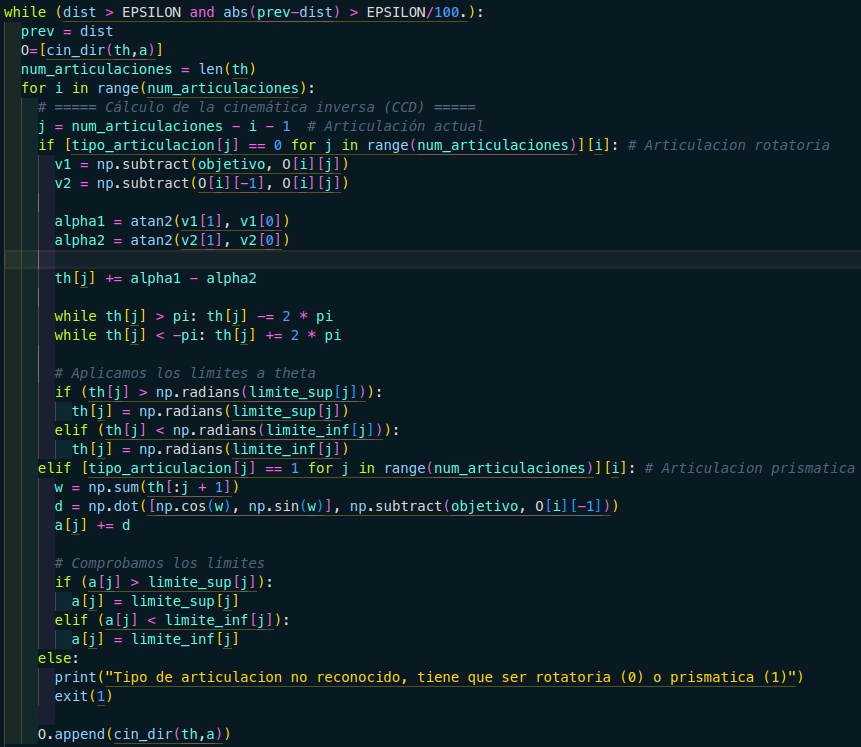
\includegraphics[scale=0.55]{img/codigo_ci_ccd.png}
  \caption{Código de la cinemática inversa con el algoritmo CCD}
\end{figure}

\newpage

\section{Ejemplo de ejecución}
Un ejemplo de ejecución del script de la cinemática inversa sería mover el robot al punto x = 5, y = 5:
\begin{figure}[H]
  \centering
  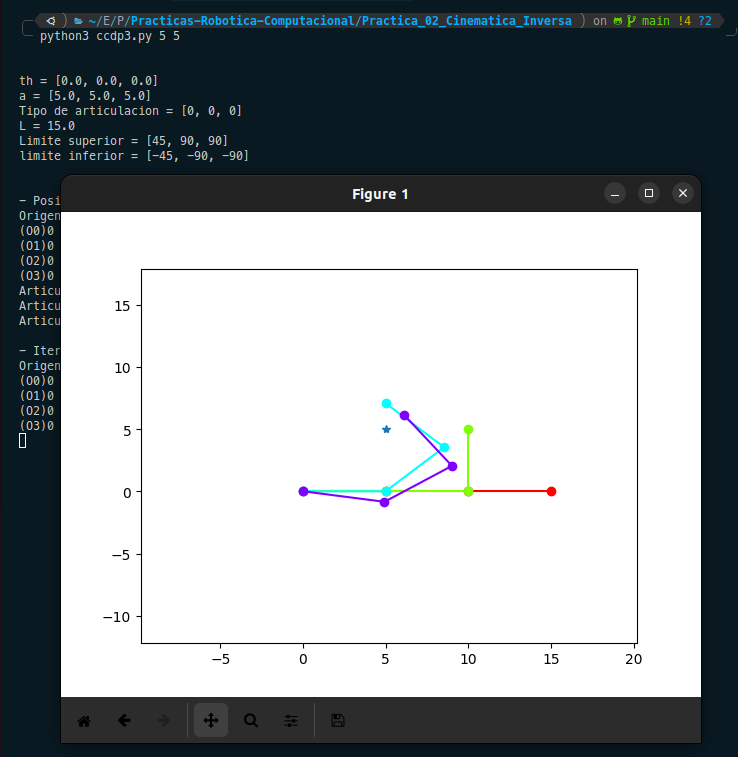
\includegraphics[scale=0.35]{img/ejemplo_ci_1.png}
  \caption{Ejemplo de ejecución de la cinemática inversa en la primera iteración}
\end{figure}

\begin{figure}[H]
  \centering
  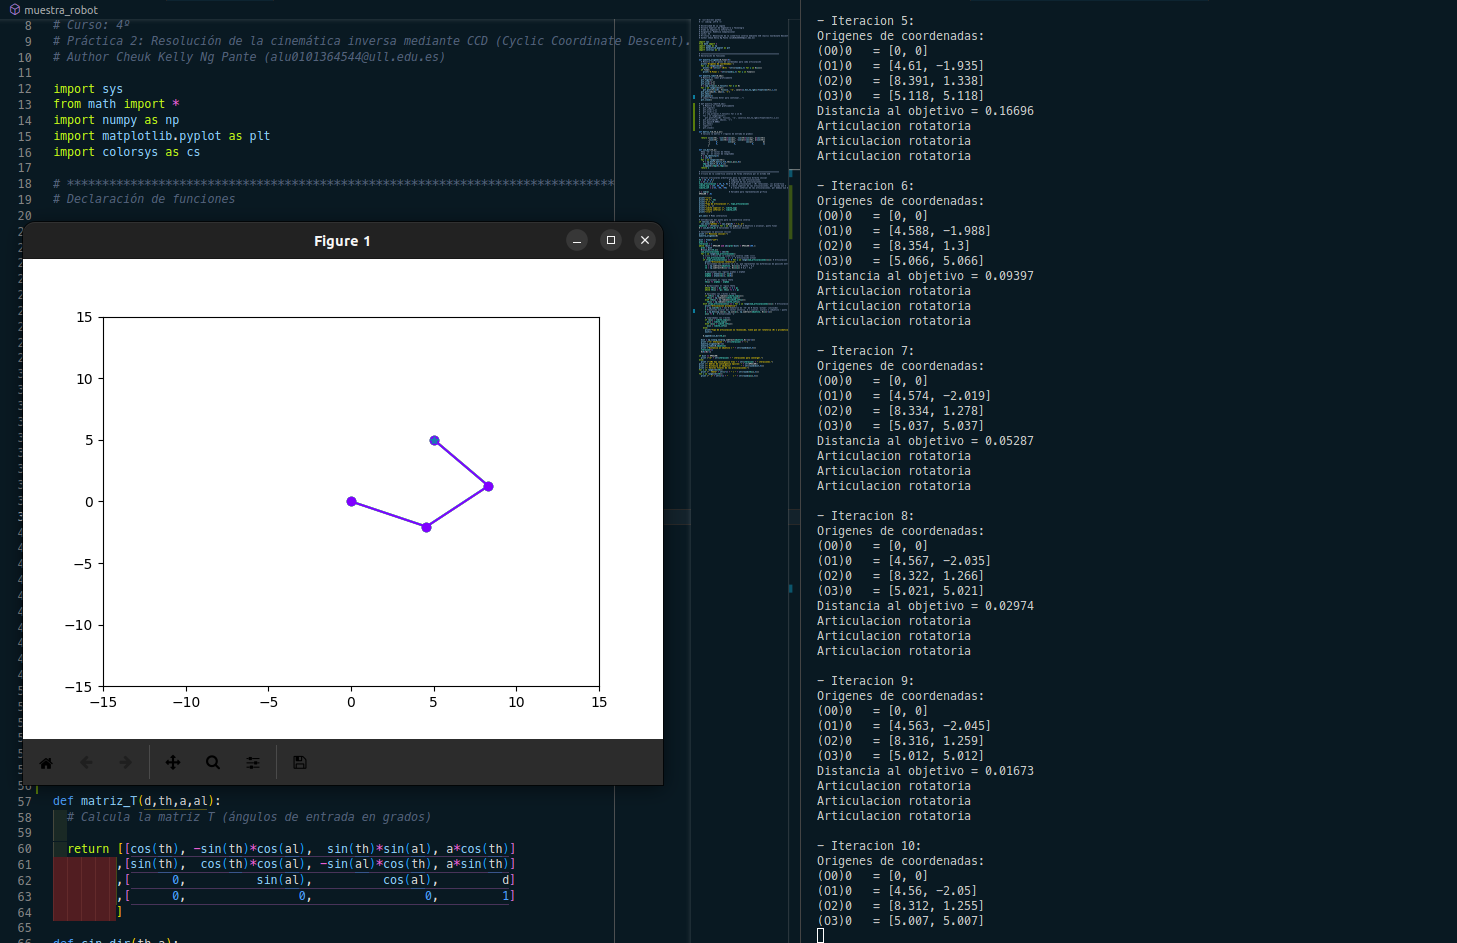
\includegraphics[scale=0.25]{img/ejemplo_ci_2.png}
  \caption{Ejemplo de ejecución de la cinemática inversa en la última iteración}
\end{figure}

\chapter{Localización}
La localización es el proceso de estimar la posición de un robot en un entorno desconocido. La localización es un problema
fundamental en la robótica móvil, ya que la mayoría de las tareas de robótica móvil requieren que el robot sepa su posición
en el entorno. La localización es un problema difícil porque el robot no conoce su posición inicial y el entorno puede ser
desconocido y dinámico. Además, los sensores del robot pueden ser ruidosos y el robot puede tener un movimiento impreciso.

En la práctica de la localización, se ha de calcular la posición más probable del robot, a partir de su sistema sensorial 
dentro de una región cuadrada de centro “centro” y lado $2 \cdot \text{radio}$.

Para calcular la localización en el script en \emph{Python} es completar la función \emph{localizacion} que recibe como parámetros
las balizas, la ubicación real del robot, la ubicación ideal del robot, el centro de la región y el radio de la región y una parametro
mostrar para mostrar el gráfico de la localización. Esta función tiene como objetivo encontrar la ubicación más probable de un robot 
dentro de una región cuadrada, utilizando su sistema sensorial y una serie de balizas de referencia.

El proceso de localización se realiza mediante la comparación de las medidas del robot real con las medidas del robot ideal en diferentes
puntos dentro de la región cuadrada. El robot ideal se mueve a cada punto y se calcula el error entre las medidas del robot ideal y las
medidas del robot real. El punto con el menor error se considera la ubicación más probable del robot real.

El código utiliza un bucle \emph{for} para iterar sobre los puntos dentro de la región cuadrada. Utiliza la función \emph{np.arange} 
para generar una secuencia de valores dentro del rango del radio de la región. Esta función devuelve un arreglo de valores que se utilizan
para calcular las coordenadas `x` e `y` del punto actual.

Dentro del bucle, se actualiza la posición del robot ideal al punto actual y se calcula el error entre las medidas del robot ideal y las 
medidas del robot real utilizando la función \emph{real.measurement\_prob(ideal.sense(balizas), balizas)}. El error se guarda en una matriz de imagen.

El código también realiza un seguimiento del error mínimo encontrado hasta el momento y el punto correspondiente a ese error mínimo. Si se 
encuentra un error menor que el error mínimo actual, se actualiza el error mínimo y se guarda el punto actual como el mejor punto.

Una vez que se completa el bucle, el robot ideal se coloca en el mejor punto encontrado, lo que se considera la ubicación más probable del 
robot real. Finalmente, se imprime el mejor punto y el error mínimo.

Una vez desarrollada la función \emph{localizacion}, se ha invocar antes de iterar sobre la lista de puntos objetivos y también al final 
para relocalizar el robot que va a calcular cual es la posición más adecuada para el robot ideal en función de la posicion del robot real.

\newpage

\section{Codigo de la localización}

\begin{figure}[H]
  \centering
  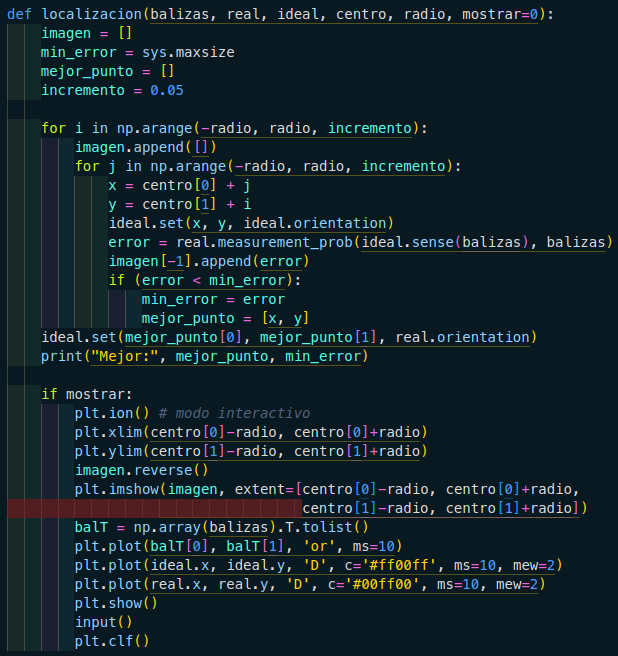
\includegraphics[scale=0.42]{img/localizacion.png}
  \caption{Código de la localización}
\end{figure}

\begin{figure}[H]
  \centering
  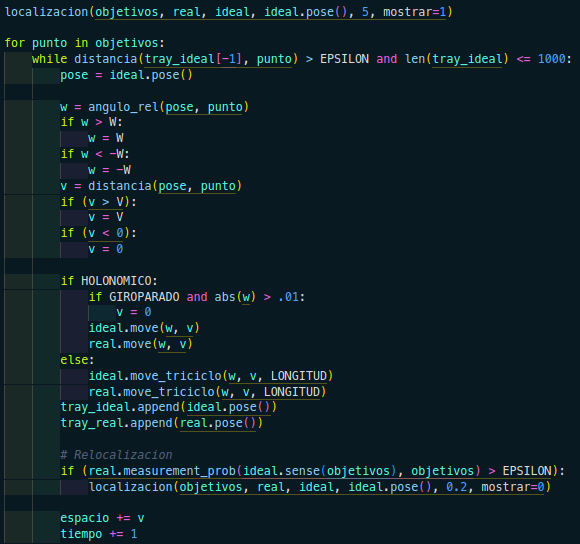
\includegraphics[scale=0.45]{img/localizacion_objetivos.png}
  \caption{Código de la localización de los objetivos}
\end{figure}

\newpage

\section{Ejemplo de ejecución}
\begin{figure}[H]
  \centering
  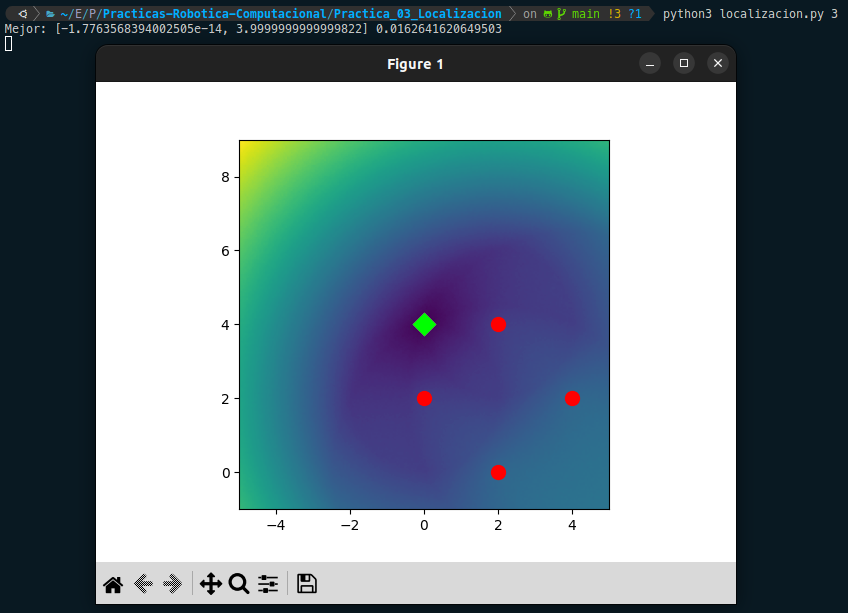
\includegraphics[scale=0.42]{img/localizacion_0.png}
  \caption{Ejemplo de ejecución de la localización}
\end{figure}

\begin{figure}[H]
  \centering
  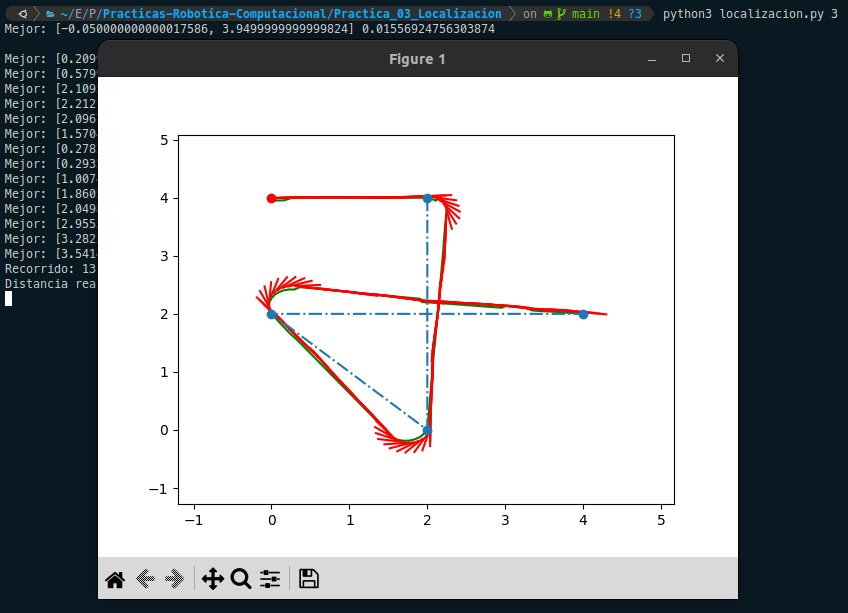
\includegraphics[scale=0.42]{img/localizacion_1.png}
  \caption{Ejemplo de ejecución de la localización}
\end{figure}

\end{document}